% d

module Chapters.Chapter4_2 where

% SINGLE_LINE e

\section{Example 2. Multiplication Table}
\label{sec:ex2}

This section shows how to describe a spreadsheet with a multiplication table. The program should produce an \texttt{xlsx} file with a multiplication table. \Cref{fig:mult} demonstrates a desired multiplication table and \Cref{fig:mult_formulas} shows the underlying formulas.

\begin{figure}[h]
  \centering
  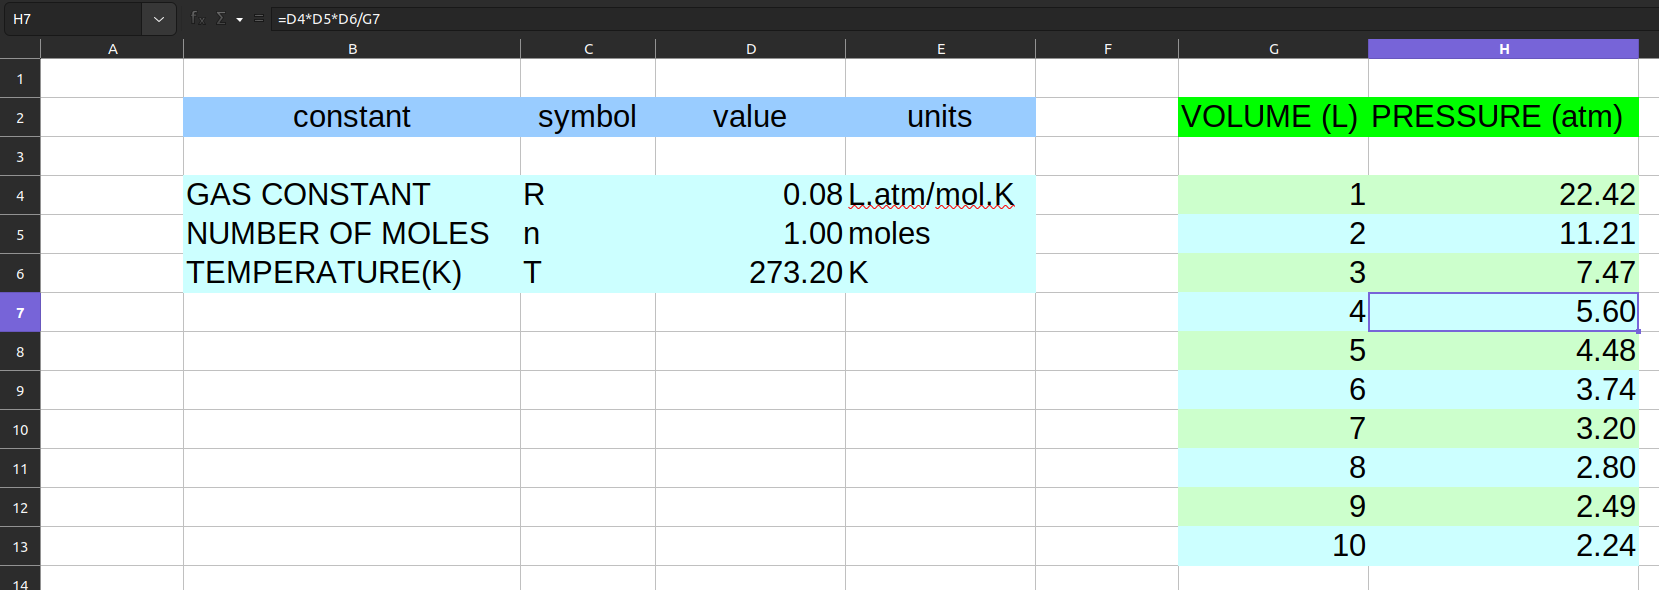
\includegraphics[scale=0.3]{demoValues.png}
  \caption{Multiplication table}
  \label{fig:mult}
\end{figure}

\begin{figure}[h]
  \centering
  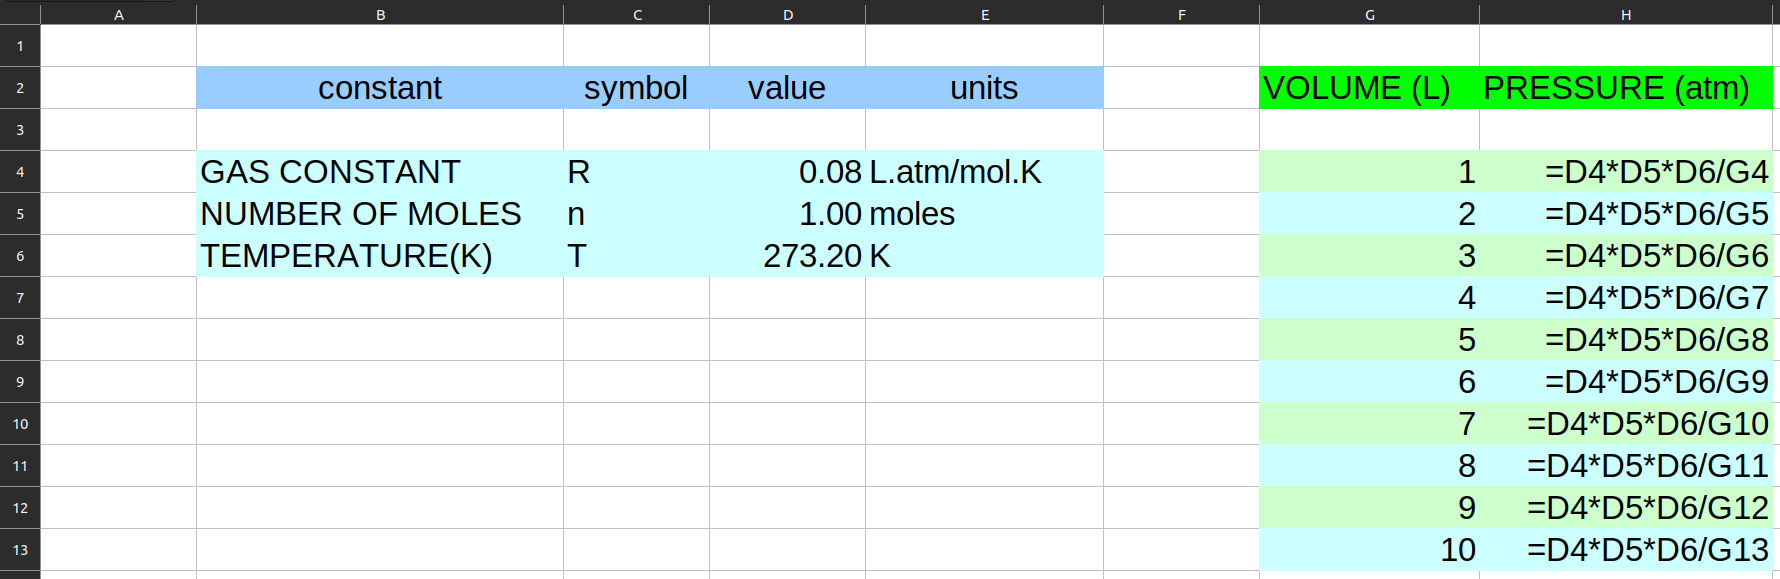
\includegraphics[scale=0.3]{demoFormulas.png}
  \caption{Multiplication table with formulas}
  \label{fig:mult_formulas}
\end{figure}

The below sections describe how such a spreadsheet can be constructed.

\subsection{Imports}

These are the necessary imports.

\begin{mycode}
import Clerk
import Control.Monad (forM, forM_, void)
import qualified Data.Text as T
import Lens.Micro ((&), (+~), (^.))
\end{mycode}

\subsection{Tables}

The tables that I construct are:

\begin{itemize}
  \item A vertical header;
  \item A horizontal header;
  \item A table with results of multiplication of the numbers from these headers.
\end{itemize}

\subsubsection{A vertical header}

\texttt{clerk} provides the \texttt{RowI} monad.
This monad takes some \texttt{i}nput, internally converts it into spreadsheet types, and outputs something, e.g., a cell reference.
In background, it writes a template of a horizontal block of cells - a \texttt{row}.
This row is used for placing the input values onto a sheet.

A vertical block of cells (\Cref{fig:vertical}) can be represented as several horizontal blocks of cells placed under each other.

\begin{figure}[h]
  \centering
  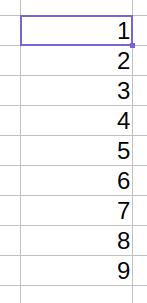
\includegraphics[scale=0.3]{vertical.png}
  \caption{A vertical header}
  \label{fig:vertical}
\end{figure}

As a template, I use a \texttt{RowI} with one integer as an input.
Because I do not need any formatting, I use \texttt{blank} cells for templates. I place the rows for each input value and collect the references.
Each row is shifted relative to the input coordinates.

\pagebreak

\begin{mycode}
mkVertical :: Coords -> [Int] -> Sheet [Ref Int]
mkVertical coords numbers =
  forM (zip [0 ..] numbers) $ \(idx, number) ->
    placeIn
      (coords & row +~ idx + 2)
      number
      ((columnF blank (const number)) :: RowI Int (Ref Int))
\end{mycode}

\subsubsection{A horizontal header}

For a horizontal header (\Cref{fig:horizontal}), I make a row of numbers and collect the references to all its cells.

\begin{figure}[h]
  \centering
  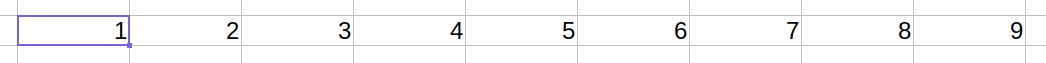
\includegraphics[scale=0.3]{horizontal.png}
  \caption{A horizontal header}
  \label{fig:horizontal}
\end{figure}

As the type of inputs is not important, I use the \texttt{Row} type.
In the \texttt{Sheet} monad, I place this row starting at a specified coordinate.

\begin{mycode}
mkHorizontal :: Coords -> [Int] -> Sheet [Ref Int]
mkHorizontal coords numbers =
  place
    (coords & col +~ 2)
    ((forM numbers $ \n -> columnF blank (const n)) :: Row [Ref Int])
\end{mycode}

\subsubsection{Table builder}

For inner cells, I use single-cell rows for each input. I place the cells as in \Cref{fig:table}.

\begin{figure}[h]
  \centering
  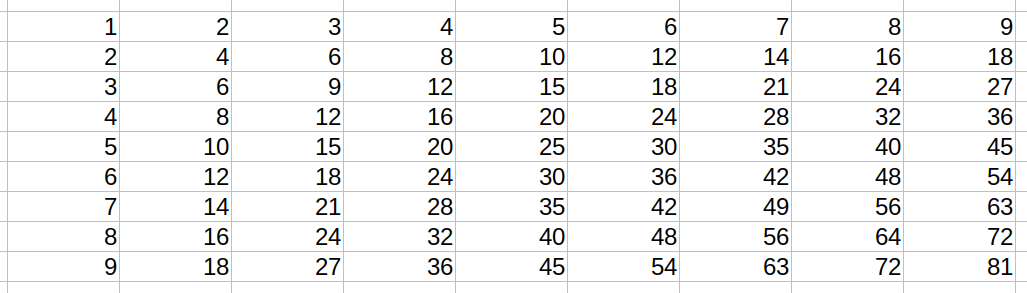
\includegraphics[scale=0.25]{table.png}
  \caption{A vertical header}
  \label{fig:table}
\end{figure}

\pagebreak
Since the information about these cells is unnecessary, I use the \texttt{Row ()} type.

\begin{mycode}
mkTable :: [(Ref Int, Ref Int)] -> Sheet ()
mkTable cs =
  forM_ cs $ \(r, c) -> do
    coords <- mkCoords (c ^. col) (r ^. row)
    place coords ((columnF_ blank (const (r .* c))) :: Row ())
\end{mycode}

\subsection{Sheet}

Here, I combine all functions to compose a complete \texttt{Sheet ()}.

\begin{mycode}
sheet :: Sheet ()
sheet = do
  start <- mkCoords 2 2
  let numbers = [1 .. 9]
  cs <- mkHorizontal start numbers
  rs <- mkVertical start numbers
  mkTable [(r, c) | r <- rs, c <- cs]
\end{mycode}

\subsection{Result}

Finally, I write the result and get a spreadsheet like the one at the beginning of this example.

\begin{mycode}
main :: IO ()
main = writeXlsx "example2.xlsx" [(T.pack "List 1", void sheet)]
\end{mycode}
